\documentclass{article}
\usepackage[utf8]{inputenc}

\title{42}
\author{Jane Doe}
\date{June 2011}

\usepackage{natbib}
\usepackage{graphicx}

push from github dj

\begin{document}

\maketitle

\section{Introduction}
There is a theory which states that if ever anyone discovers exactly what
 the Universe is for and why it is here, 
it will instantly disappear and be replaced by something even more bizarre 
and inexplicable.
There is another theory which states that this has already happened
test new github api
staging
\begin{figure}[h!]
\centering
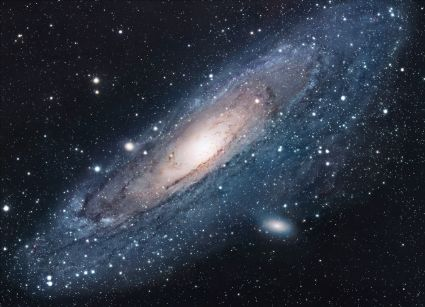
\includegraphics[scale=1.7]{universe.jpg}
\caption{The Universe}
\label{threadsVsSync}
\end{figure}

\section{Conclusion}
``I always thought something was fundamentally wrong with the universe'' \citep{adams1995hitchhiker}

\bibliographystyle{plain}
\bibliography{references}
\end{document}
